\documentclass[a4paper]{article}
\usepackage{geometry}
\usepackage{graphicx}
\usepackage{natbib}
\usepackage{amsmath}
\usepackage{amssymb}
\usepackage{amsthm}
\usepackage{paralist}
\usepackage{epstopdf}
\usepackage{tabularx}
\usepackage{longtable}
\usepackage{multirow}
\usepackage{multicol}
\usepackage[hidelinks]{hyperref}
\usepackage{fancyvrb}
\usepackage{algorithm}
\usepackage{algorithmic}
\usepackage{float}
\usepackage{paralist}
\usepackage[svgname]{xcolor}
\usepackage{enumerate}
\usepackage{array}
\usepackage{times}
\usepackage{url}
\usepackage{fancyhdr}
\usepackage{comment}
\usepackage{environ}
\usepackage{times}
\usepackage{textcomp}
\usepackage{caption}


\urlstyle{rm}

\setlength\parindent{0pt} % Removes all indentation from paragraphs
\theoremstyle{definition}
\newtheorem{definition}{Definition}[]
\newtheorem{conjecture}{Conjecture}[]
\newtheorem{example}{Example}[]
\newtheorem{theorem}{Theorem}[]
\newtheorem{lemma}{Lemma}
\newtheorem{proposition}{Proposition}
\newtheorem{corollary}{Corollary}

\floatname{algorithm}{Procedure}
\renewcommand{\algorithmicrequire}{\textbf{Input:}}
\renewcommand{\algorithmicensure}{\textbf{Output:}}
\newcommand{\abs}[1]{\lvert#1\rvert}
\newcommand{\norm}[1]{\lVert#1\rVert}
\newcommand{\RR}{\mathbb{R}}
\newcommand{\CC}{\mathbb{C}}
\newcommand{\Nat}{\mathbb{N}}
\newcommand{\br}[1]{\{#1\}}
\DeclareMathOperator*{\argmin}{arg\,min}
\DeclareMathOperator*{\argmax}{arg\,max}
\renewcommand{\qedsymbol}{$\blacksquare$}

\definecolor{dkgreen}{rgb}{0,0.6,0}
\definecolor{gray}{rgb}{0.5,0.5,0.5}
\definecolor{mauve}{rgb}{0.58,0,0.82}

\newcommand{\Var}{\mathrm{Var}}
\newcommand{\Cov}{\mathrm{Cov}}

\newcommand{\vc}[1]{\boldsymbol{#1}}
\newcommand{\xv}{\vc{x}}
\newcommand{\Sigmav}{\vc{\Sigma}}
\newcommand{\alphav}{\vc{\alpha}}
\newcommand{\muv}{\vc{\mu}}

\newcommand{\red}[1]{\textcolor{red}{#1}}

\def\x{\mathbf x}
\def\y{\mathbf y}
\def\w{\mathbf w}
\def\v{\mathbf v}
\def\E{\mathbb E}
\def\V{\mathbb V}

% TO SHOW SOLUTIONS, include following (else comment out):
\newenvironment{soln}{
	\leavevmode\color{blue}\ignorespaces
}{}


\hypersetup{
	%    colorlinks,
	linkcolor={red!50!black},
	citecolor={blue!50!black},
	urlcolor={blue!80!black}
}

\geometry{
	top=1in,            % <-- you want to adjust this
	inner=1in,
	outer=1in,
	bottom=1in,
	headheight=3em,       % <-- and this
	headsep=2em,          % <-- and this
	footskip=3em,
}


\pagestyle{fancyplain}
\lhead{\fancyplain{}{Homework 4}}
\rhead{\fancyplain{}{CS 760 Machine Learning, Fall 2021}}
\cfoot{\thepage}

\title{\textsc{Homework 4}} % Title

%%% NOTE:  Replace 'NAME HERE' etc., and delete any "\red{}" wrappers (so it won't show up as red)

\author{
	Yohei Nishimura \\
	ynishimura \\
} 

\date{}

\begin{document}
	
	\maketitle 
		
	\section*{Solution 1}
      		\subsection*{Solution 1.1: Strategy 1}
     		 \begin{soln}
		 If we $\hat{x} \in argmax_x \theta_x$, and if let j be the x at which the largest probability is taken,  then $E[1[\hat{x} = j]] = \theta_j$. Therefore, $E[1[\hat{x} \neq j]] = 1 - \theta_j$. By changing this notation j to x, we get the following equation.
 		     \[
 		     E[1[\hat{x} \neq x]] = 1 - \theta_x
 		     \]
		  \end{soln}
      
   		   \subsection*{Solution 1.2: Strategy 2}
		   \begin{soln}
  		    Suppose $\hat{x}$ is generated from a multinomial distribution. $\hat{x} = x$ because the probability of $x$ and $\hat{x}$ occurring is $\theta_x$, which is $\theta^2_x$ since the two events are independent. Therefore, we get below:
  		    \[
 		     E[1[\hat{x} \neq x]] = 1 - \theta^2_x
  		    \]
		 \end{soln}
      
      	\section*{Solution 2}
	\begin{soln}
		$E[c_{ij}]$ can be formulated as follows.
		\begin{equation*}
		\begin{split}
		E[c_{ij}] &= \frac{1}{k} (\theta_1 1[\hat{x} \neq 1] + \theta_2 1[\hat{x} \neq 2] + ... + \theta_k 1[\hat{x} \neq k] )\\
		&= \frac{1}{k} ( (1 - \theta_1) 1[\hat{x} = 1] + (1 - \theta_2) 1[\hat{x} = 2] + ... + (1 - \theta_k) 1[\hat{x} = k]  ) \\
			\end{split}
		\end{equation*}	
		In order to minimize $E[c_{ij}]$, we should choose $\hat{x}$ that minimizes the above equation. The strategy of the choice of $\hat{x}$, since we know $\theta$, we can choose the $i$ that minimizes $(1-\theta_i), i = 1, ..., k$, that is, the largest $\theta_i$ in $\theta$, as $\hat{x}$.
	
	\end{soln}
	
	\section*{Solution 3}
	\subsection*{Solution 3.1}
	\begin{soln}
	Let the mean of the distribution of $Y_t$ be $\mu$ and the variance be $\sigma^2$. In the setting of this question, since we know these two variables, the optimal strategy is to set $x_t = \mu$ at any time. It is because  $E[y_t] = \mu$, meaning that the value of $y_t$ that is most likely to appear is $\mu$.

	At this time, the expected payment for the $T$th time is as follows:
		\begin{equation*}\label{xx}
			\begin{split}
		E[T (x_t - y_t)^2] &= T (\mu^2 - 2 \mu E[y_t] + E[y_t^2)]) = T (\mu^2 - 2 \mu^2 + \sigma^2 + \mu^2) \\
		&= T \sigma^2
			\end{split}
		\end{equation*}	
During the development of the above equation, I used the following:
		\begin{equation*}\label{xx}
			\begin{split}
			Var(y_t) = \sigma^2 &= E[y_t^2] - (E[y_t])^2 = E[y_t^2] - \mu^2 \\
			\therefore E[y_t^2] &=  \sigma^2 + \mu^2
			\end{split}
		\end{equation*}	
	
	\end{soln}

	\subsection*{Solution 3.2}
	\begin{soln}
		Based on previous problem, we can set the "payment" function below:
		\begin{equation}\label{xx}
			\begin{split}
			argmin_{x_t} Payment = T ( E[x_t]^2 - 2 E[x_t] E[y_t] + E[y_t^2)])
			\end{split}
		\end{equation}	
		At the end of the $m$th enforcement, calculate the following with the realized values.
		\begin{equation*}\label{xx}
			\begin{split}
			E[x_t] &= \frac{1}{m} \sum_{i=1}^{m} x_i = \bar{x} \\
			E[x_t]^2 &= \frac{1}{m} \sum_{i=1}^{m} (x_i - \bar{x} )^2   + \bar{x}^2 = Var(x) +\bar{x}^2 \\
			E[y_t] &= \frac{1}{m} \sum_{i=1}^{m} y_i = \bar{y} \\
			E[y_t]^2 &= \frac{1}{m} \sum_{i=1}^{m} (y_i - \bar{y} )^2   + \bar{y}^2 = Var(y) +\bar{y}^2 \\
			\end{split}
		\end{equation*}	
		Then, substitute the above four equations into equation (1).
		\begin{equation}\label{xx}
			\begin{split}
			argmin_{x_t} Payment &= T ( \frac{1}{m} \sum_{i=1}^{m} (x_i - \bar{x} )^2   + \bar{x}^2 +  \frac{1}{m} \sum_{i=1}^{m} (y_i - \bar{y} )^2   + \bar{y}^2 - 2 \bar{x} \bar{y} )  \\
			&= T ( Var(x) + Var(y) + (\bar{x} - \bar{y} )^2 ) \\
			\end{split}
		\end{equation}	
		Calculate equation (2) above for the $m+1$th time as well, and if equation (2), or the benchmark, is lower than the $m$th time, we can conclude that the strategy we are currently using is correct. In other words, equation (2) is the benchmark.
	\end{soln}
	
	
	\section*{Solution 4}
	\subsection*{Solution 4.1}	
	\begin{soln}
	From the setup of this question, $N = 30$, $K_L = 3$, and $\alpha = 0.5$. Using these, calculate the prior probabilities. The total number of data is 30, e0-e9, j0-j9, s0-s9, of which 10 are in English.
		\begin{equation*}\label{xx}
			\begin{split}
				\hat{p}_{\alpha}(y = e) &= \frac{\sum_{i=1}^{N} 1[y^{(i)} = e] + \alpha }{N + K_L \alpha} \\ 
				&= \frac{10 + 0.5}{30 + 3*0.5} = \frac{1}{3}\\
			\end{split}
		\end{equation*}	
		Similarly, the two prior probabilities of ta are calculated and the answers are as follows.
		\begin{equation*}\label{xx}
			\begin{split}
				\hat{p}_{\alpha}(y = e) &= 	\hat{p}_{\alpha}(y = j) = \hat{p}_{\alpha}(y = s) =  \frac{1}{3}\\
			\end{split}
		\end{equation*}	
		
	\end{soln}
	
	\clearpage
	\subsection*{Solution 4.2}		
	\begin{soln}
	From the given conditions, calculate the following using $p(y = e) = \frac{1}{3}$.
		\begin{equation*}\label{xx}
			\begin{split}
				\theta_{i,e} = \hat{p}(c_i | y = e) = \frac{\hat{p}(c_i \cap y=e )}{\hat{p}(y=e)} = 3 \hat{p}(c_i \cap y=e ) \\
			\end{split}
		\end{equation*}		
	Then, compute the $\theta$ for each $i$. $\theta_e$ is below.
\begin{table}[ht]
 \caption{$\theta_e$}
 \centering
  \begin{tabular}{clll}
   \hline
   character & probability \\
   \hline \hline
a & 0.06 \\
b & 0.01 \\
c & 0.02 \\
d & 0.02 \\
e & 0.11 \\
f & 0.02 \\
g & 0.02 \\
h & 0.05 \\
i & 0.05 \\
j & 0.0 \\
k & 0.0 \\
l & 0.03 \\
m & 0.02 \\
n & 0.06 \\
o & 0.07 \\
p & 0.02 \\
q & 0.0 \\
r & 0.05 \\
s & 0.07 \\
t & 0.08 \\
u & 0.03 \\
v & 0.01 \\
w & 0.02 \\
x & 0.0 \\
y & 0.01 \\
z & 0.0 \\
(space)  & 0.18 \\
   \hline
  \end{tabular}
\end{table}
	\end{soln}	

	\clearpage
	\subsection*{Solution 4.3}	
	\begin{soln}
	$\theta_j$, $\theta_s$,the class conditional probabilities for Japanese and Spanish are below.

\begin{table}[h]
  \begin{minipage}[t]{.45\textwidth}
    \begin{center}
        \caption{$\theta_j$}
      \begin{tabular}{clll}
   \hline
   character & probability \\
   \hline \hline

a & 0.13 \\
b & 0.01 \\
c & 0.01 \\
d & 0.02 \\
e & 0.06 \\
f & 0.0 \\
g & 0.01 \\
h & 0.03 \\
i & 0.1 \\
j & 0.0 \\
k & 0.06 \\
l & 0.0 \\
m & 0.04 \\
n & 0.06 \\
o & 0.09 \\
p & 0.0 \\
q & 0.0 \\
r & 0.04 \\
s & 0.04 \\
t & 0.06 \\
u & 0.07 \\
v & 0.0 \\
w & 0.02 \\
x & 0.0 \\
y & 0.01 \\
z & 0.01 \\
(space)  & 0.12 \\
   \hline
      \end{tabular}
    \end{center}

  \end{minipage}
  %
  \hfill
  %
  \begin{minipage}[t]{.45\textwidth}
    \begin{center}
       \caption{$\theta_s$}
      \begin{tabular}{clll}
   \hline
   character & probability \\
   \hline \hline
a & 0.1 \\
b & 0.01 \\
c & 0.04 \\
d & 0.04 \\
e & 0.11 \\
f & 0.01 \\
g & 0.01 \\
h & 0.0 \\
i & 0.05 \\
j & 0.01 \\
k & 0.0 \\
l & 0.05 \\
m & 0.03 \\
n & 0.05 \\
o & 0.07 \\
p & 0.02 \\
q & 0.01 \\
r & 0.06 \\
s & 0.07 \\
t & 0.04 \\
u & 0.03 \\
v & 0.01 \\
w & 0.0 \\
x & 0.0 \\
y & 0.01 \\
z & 0.0 \\
(space)  & 0.17 \\
   \hline
      \end{tabular}
    \end{center}
  \end{minipage}
\end{table}
	
	\end{soln}
	\clearpage
	\subsection*{Solution 4.4}	
	\begin{soln}
	The bag-of-words vector x is below.
	\begin{table}[ht]
 \caption{x of e10.txt}
 \centering
  \begin{tabular}{clll}
   \hline
   character & numbers \\
   \hline \hline
a & 164 \\
b & 32 \\
c & 53 \\
d & 57 \\
e & 311 \\
f & 55 \\
g & 51 \\
h & 140 \\
i & 140 \\
j & 3 \\
k & 6 \\
l & 85 \\
m & 64 \\
n & 139 \\
o & 182 \\
p & 53 \\
q & 3 \\
r & 141 \\
s & 186 \\
t & 225 \\
u & 65 \\
v & 31 \\
w & 47 \\
x & 4 \\
y & 38 \\
z & 2 \\
(space)  & 498 \\
   \hline
  \end{tabular}
\end{table}
	\end{soln}

	\clearpage
	\subsection*{Solution 4.5}	
	\begin{soln}
	Taking the logarithm of the equation, we get $\log \hat{p}(x|y) = \sum_{i=1}^{d} x_i \theta_{i,y} $. Based on previous problems, $\log \hat{p}(x|y=e) = -7840.77$, $\log \hat{p}(x|y=j) = -8727.17$, and $\log \hat{p}(x|y=s) = -8478.20$, meaning $\hat{p}(x|y=e) = e^{-7840.77}$, $\hat{p}(x|y=j) = e^{-8727.17}$, and $\hat{p}(x|y=s) = e^{-8478.20}$
	\end{soln}
	
	\subsection*{Solution 4.6}	
	\begin{soln}
	Taking the logarithm of the Bayes law, we get $\log \hat{p}(y|x) = \log \hat{p}(x|y) + \log \hat{p}(y)$. Then, based on previous problems, $\log \hat{p}(y=e|x) = -7841.87$, $\log \hat{p}(y=j|x) = -8728.27$, and $\log \hat{p}(y=s|x) = -8479.30$, meaning $\hat{p}(y=e|x) = e^{-7841.87}$, $\hat{p}(y=j|x) = e^{-8728.27}$, and $\hat{p}(y=s|x) = e^{-8479.30} $. In the calculation, the results of prior probability in problem 4.2 are used.
	
	 Because $\hat{p}(y=e|x) > \hat{p}(y=s|x) > \hat{p}(y=j|x)$, it is concluded that the label of x should be "English." 
	\end{soln}
	
	\subsection*{Solution 4.7}
	\begin{soln}
	The answer table is below.
	\begin{table}[htbp]
  	\centering
	 \caption{Classification among English, Spanish and Japanese}
  	\begin{tabular}{clll}
  	    & English & Spanish & Japanese \\ 
	   \hline
  	  English & 10 & 0 & 0 \\
  	  Spanish & 0 & 10 & 0 \\ 
	  Japanese & 0 & 0 & 10 \\
 	 \end{tabular}
	\end{table}
	
	\end{soln}
	
	\subsection*{Solution 4.8}
	\begin{soln}	
	Shuffling the order of the letters does not affect the results of the estimation using this Naive Bayes classifier’s prediction. This is because the order information has been omitted when creating the bag-of-words for each training and validation data, i.e. mathematically, when calculating the likelihood.
	\end{soln}
	
	
	\section*{Solution 5}
	\subsection*{Solution 5.1}	
	\begin{soln}
	Set $z$ as $z = W_2 \sigma(W_1 x)$ and $\delta_{i,j} = 1 ($when $i=j)$, $0$ otherwise.
		\begin{equation*}\label{xx}
			\begin{split}
\frac{\partial L}{\partial W_2} &= \frac{\partial L}{\partial \hat{y}} \frac{\partial g(z)}{\partial z} \frac{\partial z}{\partial W_2} \\
				&= - \sum^{k}_{i=1} \frac{y}{\hat{y}} y_i (\delta_{i,j} - y_j) \sigma(W_1 x ) \\
				&= (\hat{y} - y) \sigma(W_1 x ) \\
				\\
\frac{\partial L}{\partial W_1} &= \frac{\partial L}{\partial \hat{y}} \frac{\partial g(z)}{\partial z} \frac{\partial z}{\partial \sigma(W_1 x)} \frac{\partial \sigma(W_1 x)}{\partial W_1 x} \frac{\partial W_1 x}{\partial W_1}   \\
				&= - \sum^{k}_{i=1} \frac{y}{\hat{y}} y_i (\delta_{i,j} - y_j) W_2 \sigma(W_1 x) (1-\sigma(W_1 x) x \\
				&= (\hat{y} - y) W_2 \sigma(W_1 x) (1-\sigma(W_1 x) x \\
			\end{split}
		\end{equation*}	
		
	\end{soln}
	
	\clearpage
	
	\subsection*{Solution 5.2}	
	\begin{soln}
	The number of epoch( = iteration / batch\_size) is 30. The final test error ( = 1 - accuracy ) is 0.0839. Learning curve by loss and the history of error are below.
\begin{figure}[htbp]
\begin{minipage}{0.5\hsize}
\begin{center}
\caption{Learning curve by my model}
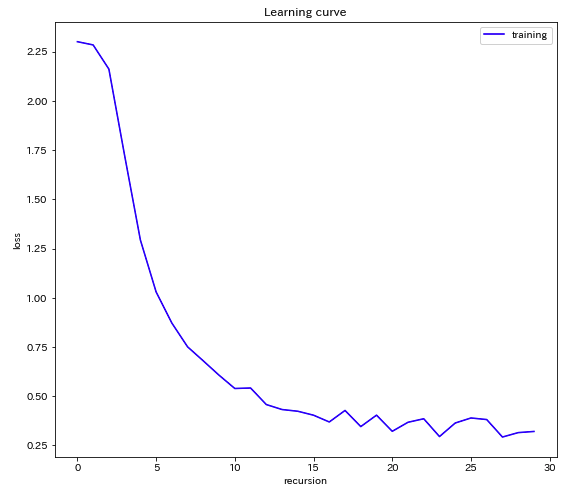
\includegraphics[width=50mm]{./img/my_learningcurve.png}
\end{center}
\captionsetup{labelformat=empty}
\end{minipage}
\begin{minipage}{0.5\hsize}
\begin{center}
\caption{Test error by my model}
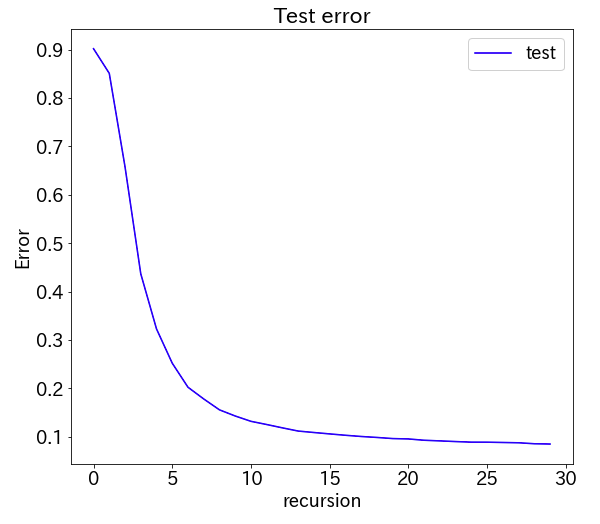
\includegraphics[width=50mm]{./img/my_testerror.png}
\end{center}
\captionsetup{labelformat=empty}
\end{minipage}
\end{figure}
	\end{soln}

	\subsection*{Solution 5.3}	
	\begin{soln}
	The number of epoch is 30. The final test error is 0.0352. Learning curve by loss and the history of error are below.
\begin{figure}[htbp]
\begin{minipage}{0.5\hsize}
\begin{center}
\caption{Learning curve by pytorch model}
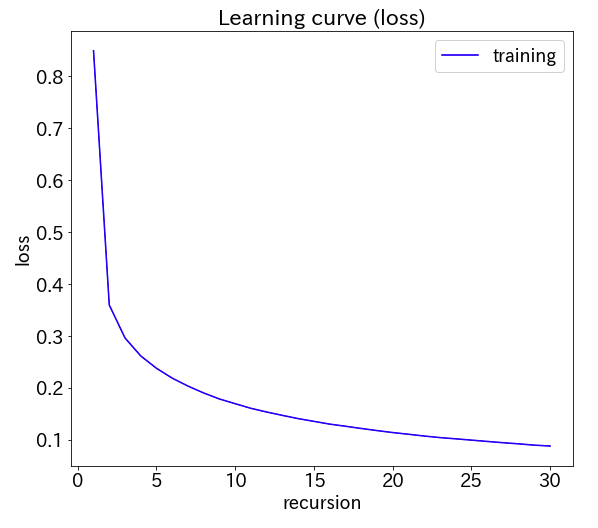
\includegraphics[width=50mm]{./img/pytorch_learningcurve.png}
\end{center}
\captionsetup{labelformat=empty}
\end{minipage}
\begin{minipage}{0.5\hsize}
\begin{center}
\caption{Test error by pytorch model}
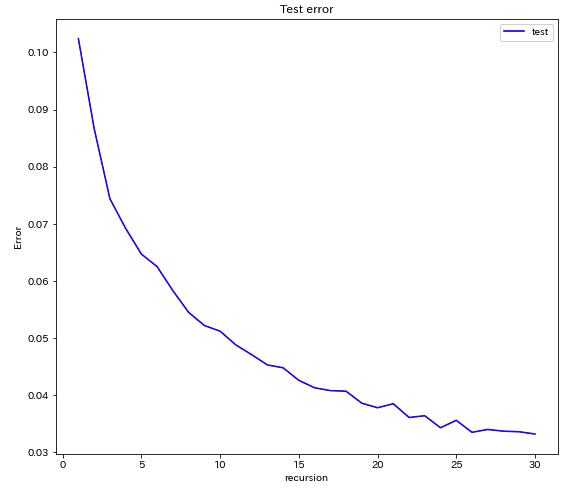
\includegraphics[width=50mm]{./img/pytorch_testerror.png}
\end{center}
\captionsetup{labelformat=empty}
\end{minipage}
\end{figure}

	\end{soln}
	
	\clearpage
	
	\subsection*{Solution 5.4.a}	
	\begin{soln}
	The number of epoch is 30. The final test error is 0.8865. Learning curve by loss and the history of error are below.
\begin{figure}[htbp]
\begin{minipage}{0.5\hsize}
\begin{center}
\caption{Learning curve by my model (zeros) }
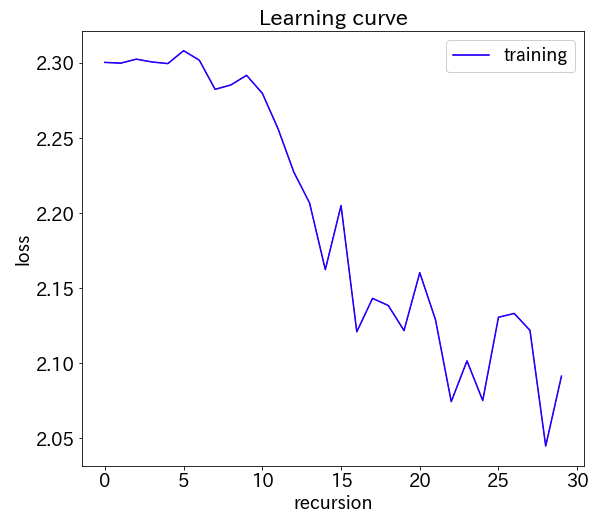
\includegraphics[width=50mm]{./img/my_lc_a.png}
\end{center}
\captionsetup{labelformat=empty}
\end{minipage}
\begin{minipage}{0.5\hsize}
\begin{center}
\caption{Test error by my model (zeros) }
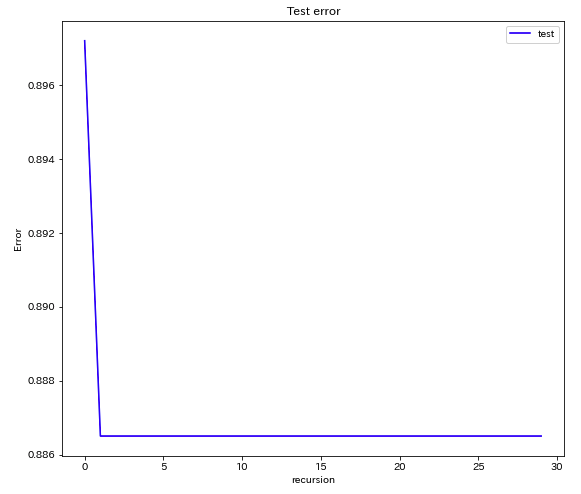
\includegraphics[width=50mm]{./img/my_er_a.png}
\end{center}
\captionsetup{labelformat=empty}
\end{minipage}
\end{figure}
	\end{soln}

	\subsection*{Solution 5.4.b}
	\begin{soln}
	The number of epoch is 30. The final test error is 0.1102. Learning curve by loss and the history of error are below.
\begin{figure}[htbp]
\begin{minipage}{0.5\hsize}
\begin{center}
\caption{Learning curve by my model (random) }
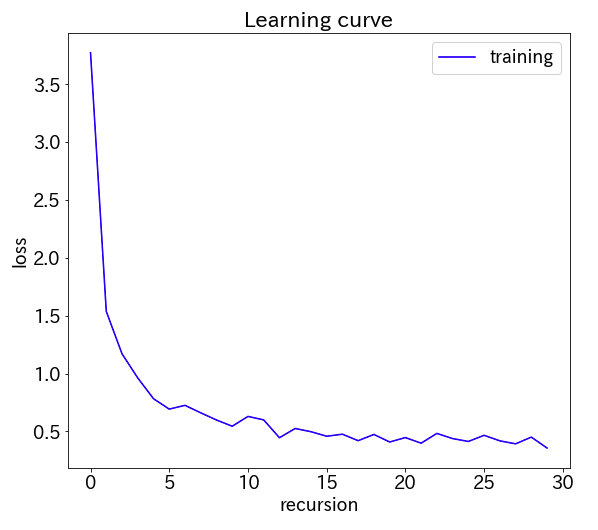
\includegraphics[width=50mm]{./img/my_lc_b.png}
\end{center}
\captionsetup{labelformat=empty}
\end{minipage}
\begin{minipage}{0.5\hsize}
\begin{center}
\caption{Test error by pytorch model (random) }
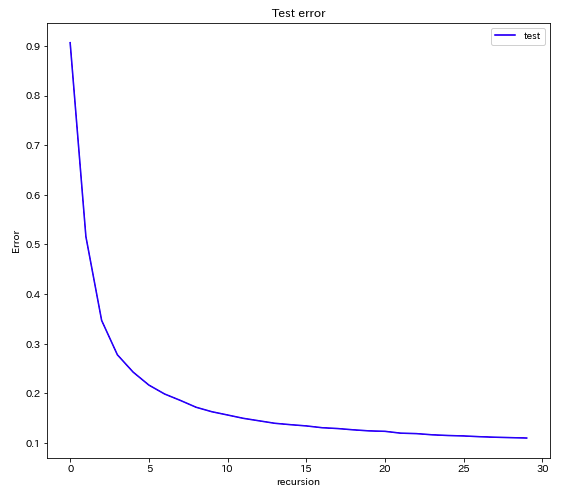
\includegraphics[width=50mm]{./img/my_er_b.png}
\end{center}
\captionsetup{labelformat=empty}
\end{minipage}
\end{figure}

	\end{soln}

		
\bibliographystyle{apalike}
	
		
	
	
	
	
	
	
	
	
	
	
\end{document}
